\chapter{Application concept}

This chapter describes the project plan and the concepts for the developed application. These concepts are foundation of the developed application and describe how the internal processes in the application work.


\section{Project planning}

First step for this project was analyzing the features from existing cost estimation software as described in section \ref{sec:stateofart}. \\
The next step was creating a GUI prototype to show how the estimation would look like on a smartphone.\\
The definition of the wanted features for the application was done regular meetings with my supervisor Prof. Dr. Georg Rock. Those features request were compiled into the project goals and requirements. The development were performed with the iterative method, where the set project steps where performed and in a meeting reviewed. This resulted in the next iteration step and further requirements.

\subsection{Objectives}\label{objectives}

The project targets are the benefit the application should bring the user. They are linked with the requirements from section \ref{requirements} and describe the condition to be achieved with the application. Whereas requirements can change over time, targets stay the same.\\
Most important target, as described in table \ref{projecttargets}, is T01. 'The application must allow a quick and mobile cost estimation of IT Projects' describes that the cost estimation has to be implemented for mobile device use. Also, the cost estimation has to be fast and can use features of the mobile platform to achieve this target.\\
As the developed application is only a beta version, it has to be developed modular for future feature implementation, as described in T04.\\
T06 describes the target that represents an admired feature. The application should provide the possibility to compare projects and measure their relation. This allows to check previous projects for their cost estimation, that the user has a reference how much effort similar projects took.\\
The target for this bachelor thesis is to implement the function point estimation technique. This is the showcase for this application and shows the possibility of cost estimations for software project on mobile devices and is described in T09.\\
All remaining targets are medium priority and describe what processes to achieve with this project.\\

\begin{table}[h]
	\centering 
	\setlength{\tabcolsep}{4pt}
	\begin{tabular}{|l||p{14cm}|}\hline
		ID		& Target\\ \hline\hline
		T01  	& The application must allow a quick and mobile cost estimation of IT Projects.\\ \hline
		T02  	& The application must provide informations how cost estimations work.\\ \hline
		T03  	& The application have to improve the cost estimation during  the project life cycle.\\ \hline
		T04  	& The application architecture has to be modular to add new cost estimation methods and analysis tools faster and more efficient.\\ \hline
		T05  	& With the application it is possible to get the information of completed projects and take advantage of their estimation.\\ \hline
		T06  	& The application allows comparison between projects and shows projects that are related to each other.\\ \hline
		T07  	& The application gives information about the estimated man days of a project and the estimated costs.\\ \hline
		T08  	& A project analysis within the application allows an overview of the project changes and gives detailed information about the estimation.\\ \hline
		T09  	& Till the end of the bachelor thesis the function point method has to be implemented and be fully operational.\\ \hline
	\end{tabular} 
	\caption{Project Targets} 
	\label{projecttargets} 
\end{table}

\subsection{Requirements}\label{requirements}

All requirements for the implemented application are based on the targets from section \ref{objectives} and the regular meetings. Those are all implemented in the developed application. This section describes the requirements for project creation in detail. All other requirements can be found in the appendix.\\
Table \ref{projectrequirementsprojectcreation} describes the requirements for the project creation. As most features in the application work with projects, those are one of the most important requirements. The requirements make sure that projects are created correctly and allow the algorithm for related project to find all projects that are related.\\

\begin{table}[h]
	\centering 
	\setlength{\tabcolsep}{4pt}
	\begin{tabular}{|l||p{5cm}|p{9cm}|}\hline
		ID		& Title&Description\\ \hline\hline
		R022  	& Create Project&It is possible to create an new project in the application\\ \hline
		R023  	& Create Project: Project Name
		&To create a Project a new Name must set
		\\ \hline
		R024 	& Create Project: unique ID
		&All Projects have an unique ID.
		\\ \hline
		R025  	& Create Project: Set Estimation Method
		&To create a Project an available estimation method must be set
		\\ \hline
		R026  	& Create Project: Load Project Influence Factors
		&After an Estimation Method is set the influencing factors are loaded
		\\ \hline
		R027  	& Create Project: Set Influencing Factors
		&All Influence Factors need to be set to complete the creation process
		\\ \hline
		R028  	& Create Project: Project Phase
		&For the creation Process the actual Project Phase must be set
		\\ \hline
		R029  	& Create Project: Project Properties
		&There has to be the possibility to add existing project documents
		\\ \hline
		R030  	& Create Project: Development Market
		&The development market of the Project is selectable 
		\\ \hline
		R031  	& Create Project: Development Kind
		&The development kind of the Project is selectable 
		\\ \hline
		R032  	& Create Project: Process Methology
		&The process methology of the Project is selectable 
		\\ \hline
		R033  	& Create Project: Programming Language
		&The programming language of the Project is selectable 
		\\ \hline
		R034  	& Create Project: Platform
		&The platform of the Project is selectable 
		\\ \hline
		R035  	& Create Project: Industry Sector
		&The industry sector of the Project is selectable 
		\\ \hline
		R036  	& Create Project: Architecture
		&The architecture of the Project is selectable 
		\\ \hline
		R037  	& Create Project: Project Icon
		&The project icon is selectable 
		\\ \hline
		R038  	& Create Project: Guided Creation Process
		&It is possible to start a guided creation for the project which guides the user through each step
		\\ \hline
		R039  	& Create Project: List Creation
		&It is possible to create a new project with a list creation which inherits all properties for the creation
		\\ \hline
		R040  	& Create Project: Long Project Name
		&Project names have to be limited to 40 characters
		\\ \hline
		R041  	& Create Project: Preselected Properties
		&One value must be preselected for all properties.
		\\ \hline
		R042  	& Create Project: Description
		&It should be possible to add a project description
		\\ \hline
		R043  	& Create Project: Property Sorting
		&All Properties are sorted alphabetically descending for the selection
		\\ \hline
	\end{tabular} 
	\caption{Project Creation Requirements} 
	\label{projectrequirementsprojectcreation} 
\end{table}

\subsection{Cost Estimation}
For the evaluation of the needed time, the project was estimated with the function point technique. Therefor all functionalities are grouped into functional groups, as described by Poensgen \cite{FPKompakt}. Afterwards each function was assigned a category for the estimation, as described in \ref{fpcomponents}.\\
The group Project, as described in \ref{fig:projectFunctionalityGroup}, inherits all functions for a project. All function groups for the application can be found in the application.
The project functionalities in \ref{fig:projectFunctionalityGroup} are created with the requirements. Some requirements can be grouped into one functionality. As an example the function Create/Edit project inherits all requirements described in table \ref{projectrequirementsprojectcreation}. This function is marked as an EI and ILF because all changes are made by the user for this function and creates or edit all internal files for the project. \\
Functions that expects an input from the user are marked as EI, like delete project. Output functions like show estimated cost are a EO function, because they only display values and results to the user. Functions with a calculation are described as EQ combined with EO if they produce an output like Export Project or process an Input like Change Estimation.
\\
\begin{figure}[h] 
	\centering 
	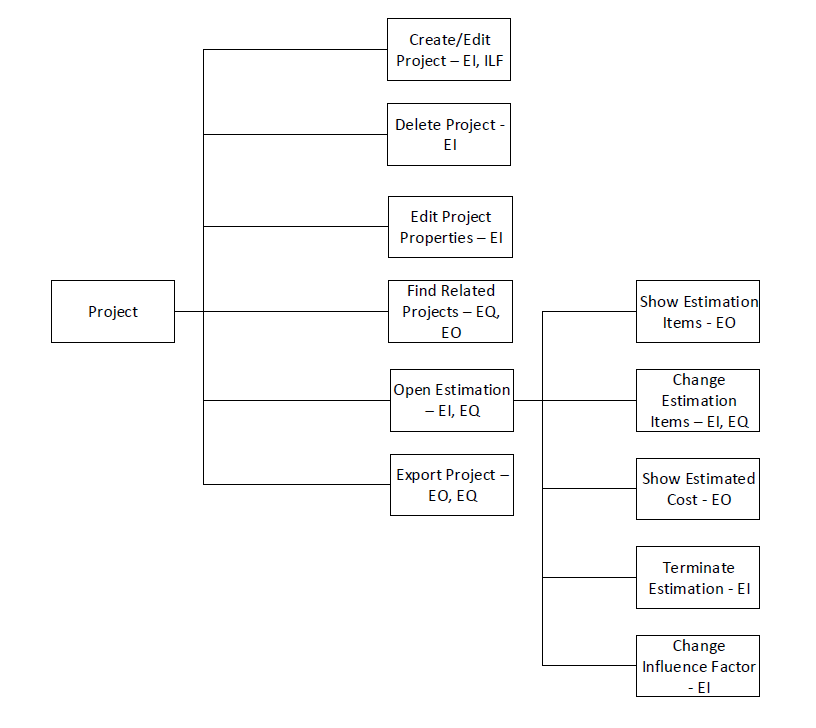
\includegraphics[width=14cm]{images/ScreenOverviewProject.PNG} 
	\caption{- Project Functionality Group} 
	\label{fig:projectFunctionalityGroup}
\end{figure}\\
Summed up the project has total 246 function points. The total functional group can be found in the appendix. \\
As described in section \ref{FPMethod}, the next step is to set the influence factors. There is no direct communication between the application and other software. It uses some functionalities for sending data to other applications, which is the reason why the influence factor 'Integration into other applications' is set to 2.
Completed with the equation from \ref{FPMethod} the influence factor multiplier is 0.99. 
\\
The complete equation of the estimation results in 243.54 points. Calculated with the points per day from table \ref{tab:pointsperday} the project is estimated to take 14 days.

\begin{figure}[h] 
	\centering 
	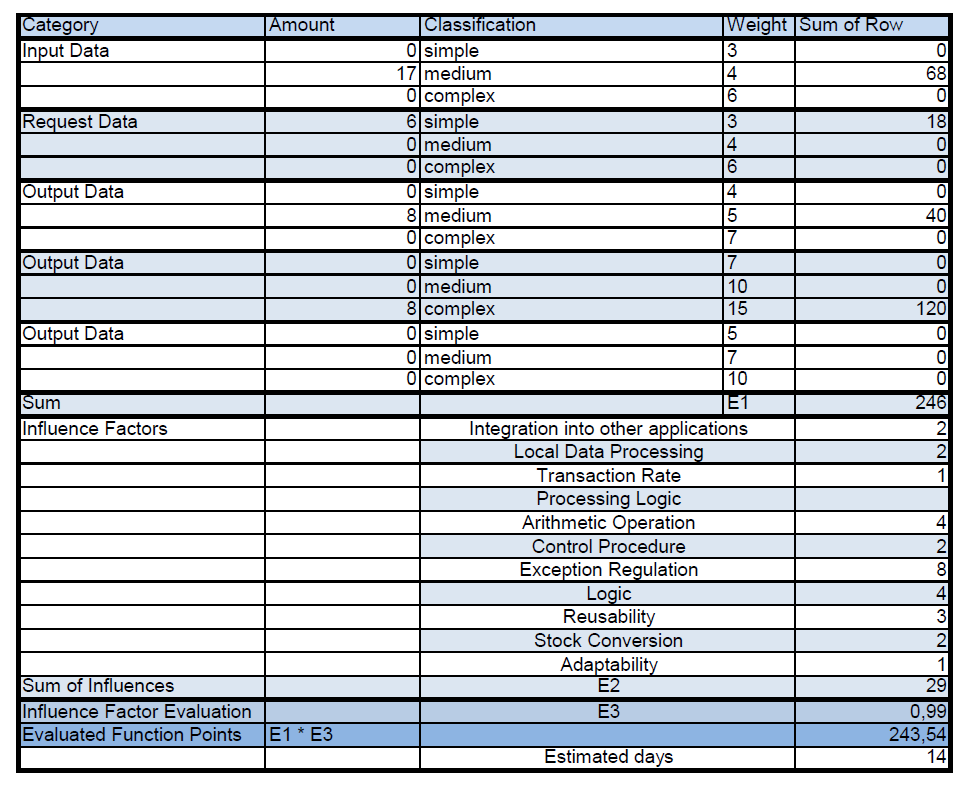
\includegraphics[width=14cm]{images/mobileestimatEstimation.PNG} 
	\caption{- MobileEstimate - Function Point Estimation} 
	\label{fig:projectEstimation}
\end{figure}

\section{Architecture}

Schaubild zur Architektur der Anwendung, einzelne Punkte besprechen

\section{Components}

Beschreibung in Welche Komponenten die Anwendung aufgeteilt ist.

\subsection{Database Helper}

Alle SQL Befehle werden über diese Klasse gemacht. Muss in allen Klassen die Zugriff auf die Datenbank haben wollen eingebunden werden. Befehle zu großen Teilen sehr Abstrakt gehalten

\subsection{Influence Factors}

Kompontene mit den Einflussfaktoren entsprechend der gewählten Schätzmethode. Summe Aller Faktoren zur Berechnung mit den Punkten der Schätzmethode

\subsection{Projekt Daten}

Speicherung aller benötigten Daten in einer Klasse. Properties und Einflussfaktor in eugener Klasse und als Objekt in Projekt vorhanden

\subsection{Related Project}

Berechung der Relevanz verschiedener Projekte. Eingehen auf die Grundlage hierfür und Beschreibung der Berechnung 

\subsection{Weitere Features}

Export, statistic, Help DB, Feedback, Project Filter, Analysis


\section{Database design}

Vorheriges Design der zentralen Datenbank. Wichtig um die Klassen anzupassen und vorher schon mit wichtigen Daten zu füllen

\subsection{Project Database}

Datenbank für alle Projekte, Eigenschaften, Einflussfaktoren

\subsubsection{Project Properties}

Welche Tabellen gibt es. Wichtige Tabellen, Aufbau der Tabellen und Grund

\subsubsection{Influence Factors}

Wie die Einflussfaktoren Aufgebaut, was ist der Gedanke dazu?

\subsubsection{Projects}

Wie sind Projekte gespeichert, Aufteilung in Projekt, Projektdetails und zugehörige Tabellen, wie die Schätzung Organisiert und wie der Zugriff auf die Elemente

\subsection{Userinformation Database}

Datenbank für Spätere Synchronisation und Userinformationen vom Server, Konzept dazu

\section{User Interface}

\subsection{Projects Overview}

Anordnung der Projekte, Wichtige Informationen zum sehen, Filtern und Suchen nach Projekten

\subsection{Project Creation}

Komponente zur korrekten Erstellung von Projekten, Geführte Eingabe, Korrekte Erstellung von Projekten in der DB, Swipe Funktion

\subsection{Estimate Function Point Project}

Aufbau der Schätzung, Umwandlung von Tabelle in App

\subsection{Influence Factors}

Aufbau der EInflussfaktoren, Neue anlengen

\subsection{Analysis}

Wie die Analyse aufgebau und was soll diese bringen?

\section{Adjusted Estimation Process}


